\section{Introduction}\label{chp4:intro}

Long term vapor intrusion (VI) studies in both residential and larger commercial structures have raised concerns regarding significant observed transient behavior in indoor air contaminant concentrations\cite{u.s._environmental_protection_agency_oswer_2015,folkes_observed_2009,holton_temporal_2013,johnston_spatiotemporal_2014,hosangadi_high-frequency_2017,mchugh_recent_2017,u.s._environmental_protection_agency_assessment_2015}, a phenomena that has previously been observed at houses impacted by radon intrusion\cite{hubbard_time-variation_1996}.
Such variations make it difficult for those charged with protecting human health to formulate a response and appropriate risk evaluation.
Furthermore there is uncertainty within the VI community regarding how to best develop sampling strategies to address this problem\cite{u.s._environmental_protection_agency_oswer_2015,holton_temporal_2013,johnson_integrated_2016,mchugh_recent_2017}.\par

To address these concerns, the EPA purchased two VI impacted houses and outfitted them with a wide variety of sensors and sampling instrumentation to study VI at these houses in great detail.
Indoor contaminant concentration as well soil-gas and groundwater contaminant concentration at different depths and locations were recorded, while simultaneously recording metrics such as indoor and outdoor temperature, wind speed and direction, and building pressurization.
These measurements were taken continuously over multiple years an unprecedented detailed dataset for exploring VI.\par

One of these houses was in Layton, Utah, near Hill AFB, and was purchased in collaboration with a research group at Arizona State University (ASU), who conducted most of the research at the site - this site will be referred to as the "ASU house" throughout this work\cite{holton_temporal_2013}.
The other was in duplex in Indianapolis, Indiana, and will be referred to as the "EPA duplex".
There work was not primarily isolated to one group.\par

One thing both of these sites had in common was that after a few years of study, preferential pathways were discovered at the sites.
A preferential pathway is typically thought of as some conduit that can transport large amounts of contaminant vapors into a building, in contrast with the slower vapor transport in soils.\par

At the ASU house, this took the form of a land drain underneath the house foundation, presumably to drain excess water from the sub-slab region.
This land drain was connected to the nearby sewer and exited into a gravel layer under the foundation, near a breach in the slab.
The sewer was buried deep enough to be partially submerged in the TCE contaminated groundwater, which likely infiltrated into the sewer.
The land drain was later excavated and fitted with a valve, allowing the researchers to control its influence - which was revealed to be very significant\cite{guo_identification_2015}.
The details of this is covered further down.\par

At the EPA duplex, the sewer acted as a preferential pathway, somewhat similar to the ASU house, but the nature of this preferential pathway was quite different from the one at the ASU house.
A tracer gas test demonstrated that contaminant vapors were directly transported into the duplex\cite{mchugh_evidence_2017}; similar to a site in Boston, Massachusetts, where PCE was transported into a bathroom through broken plumbing fixtures\cite{pennell_sewer_2013}.
It was also demonstrated that contaminated groundwater infiltrated the sewer a few blocks away from the duplex, where a dry-cleaners had  previously been.
This type of distributed contamination via a sewer network has likewise been recorded in Denmark\cite{nielsen_remediation_2017} as a VI source - giving rise to a very different situation compared to radon intrusion.\par

It is also likely that the sewer pipe at the duplex leaked contaminant vapors somewhere near the vicinity of the house.
This would give a situation that is similar to the ASU house land drain, but somewhat mitigated since the pipe leakiness is likely due to structural degradation, e.g. cracks in the mantle area; quite different from open channel flow from the ASU house land drain.\par

These works shows some of the diverse ways that a preferential pathway can play a role in VI (Figure \ref{fig:preferential_pathway_cartoon} shows a visual summary of these ways), and our poor understanding in evaluating their significance.
However, since the influence of the preferential pathway at the ASU house was able to be turned on and off (via the valve), we have an unprecedented opportunity to explore the effects of such a preferential pathway at a VI site.\par

\begin{figure}[htb!]
  \centering
  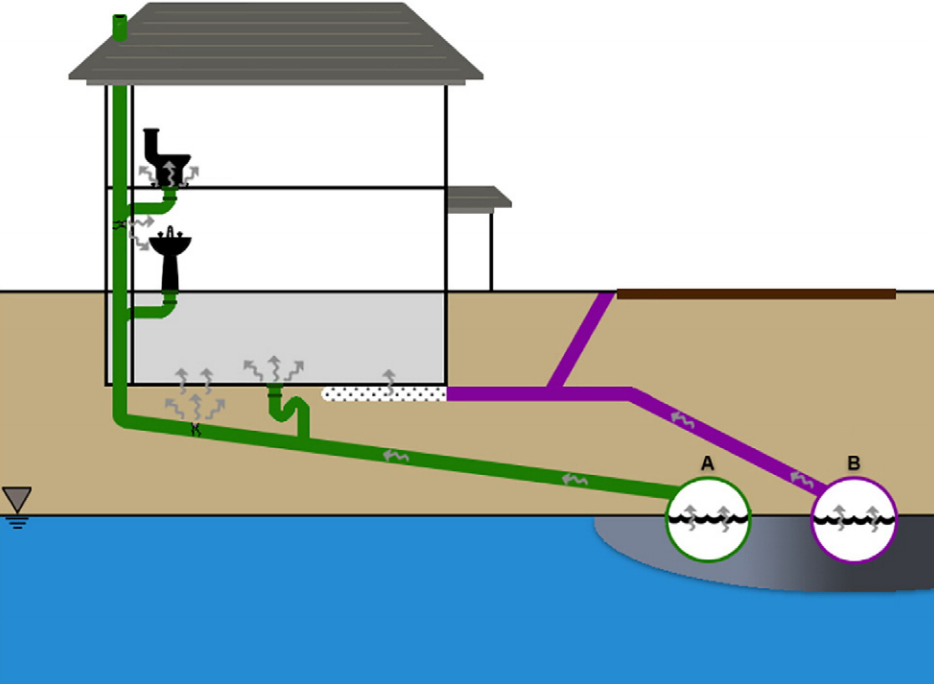
\includegraphics[width=0.75\textwidth]{preferential_pathway_cartoon.png}
  \caption{Visual summary of some of the different ways that contaminant infiltration, and ultimate transport into a VI affected building. Figure from \citeauthor{mchugh_evidence_2017}\cite{mchugh_evidence_2017}.}
  \label{fig:preferential_pathway_cartoon}
\end{figure}

\subsection{The ASU House}

The VI study at the ASU house had primarily two purposes:
\begin{enumerate}
  \item Investigate VI with a particular focus on understanding the temporal and spatial variability.
  \item Test and evaluate the performance of the controlled pressure method (CPM).
\end{enumerate}\par

This was to be achieved by monitoring various metrics relevant to VI, such as building pressurization, air exchange rate, indoor and outdoor temperature, and other metrological variables, while simultaneously monitoring the indoor air contaminant concentration.
Additionally, soil-gas and groundwater contaminant concentration underneath and around the house were monitored; the specific sampling locations, as well as a photo of the house, can be seen in Figure \ref{fig:asu_house}.
The study of the ASU house is one of the most detailed studies of a VI site to date and fully describing the experimental setup and measured metrics is beyond the scope of this work but is detailed in \citeauthor{holton_temporal_2013}\cite{holton_temporal_2013}.\par

\begin{figure}[htb!]
  \centering
  \begin{subfigure}[t]{0.45\textwidth}
    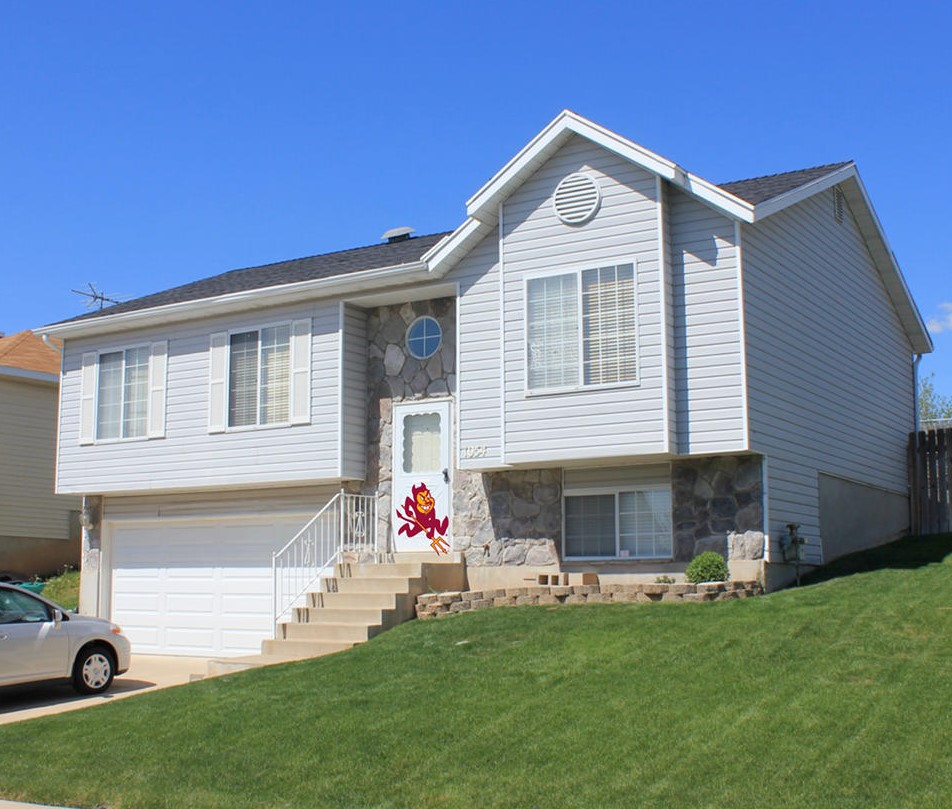
\includegraphics[width=\textwidth]{asu_house.jpg}
    \caption{Picture of the "ASU house" from \citeauthor{holton_temporal_2013}\cite{holton_temporal_2013}}
    \label{fig:asu_house}
  \end{subfigure}
  \begin{subfigure}[t]{0.50\textwidth}
    \centering
    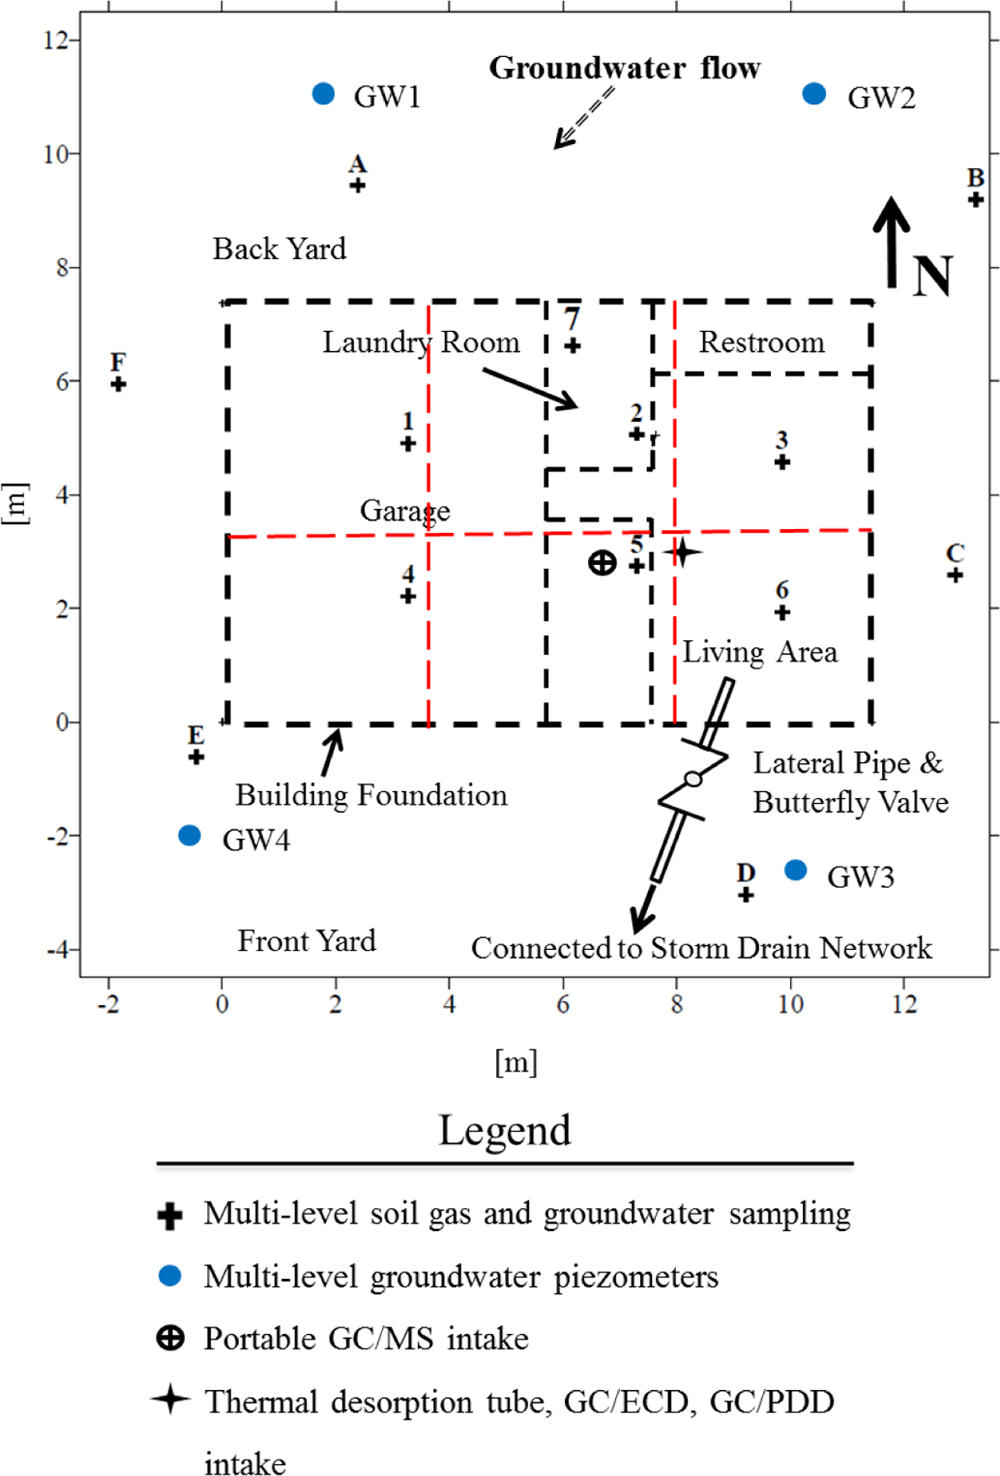
\includegraphics[width=\textwidth]{land_drain_location.jpg}
    \caption{Floor plan of the "ASU house". Locations of all sampling ports and of the land drain preferential pathway marked. Figure from \citeauthor{guo_identification_2015}\cite{guo_identification_2015}.}
    \label{fig:land_drain_location}
  \end{subfigure}
\end{figure}

CPM seeks to control the pressurization of the building, and thereby controlling the contaminant entry rate.
In this framework, overpressurizing a building will eliminate contaminant entry rate into the building, thereby identifying indoor contaminant sources.
By contrast, depressurizing a building will increase contaminant entry rate, giving a theoretical "worst-case" VI scenario.
Here the researchers would use a 20 inch window box fan to control the pressurization of the building.\par

The site was monitored for roughly 1.5 years before the testing of the CPM system commenced.
During this time, it was established that the indoor contaminant concentration fluctuated significantly at the site - roughly an order of magnitude on a weekly basis, while up to three or more orders of magnitude on a seasonal basis.
Once the house was depressurized using the CPM system, indoor contaminant concentration increased to higher concentration levels previously recorded - an initial verification of the CPM framework\cite{holton_long-term_2015}.\par

However, during the CPM testing period, the researchers noticed that the house and nearby sewer seemingly communicated with each other.
This was shown by the movement of a plastic tarp, which covered a nearby manhole, as the door of the house was opened and closed.
This lead to the discovery of the land drain preferential pathway at the site; the location of it in relation to the house floorplan can be seen in Figure \ref{fig:land_drain_location}
The land drain determined to exit into the gravel sublayer beneath the foundation, near a visible breach in the foundation slab, and was subsequently excavated and fitted with a butterfly valve \cite{guo_identification_2015} to control its influence.\par

\begin{figure}[htb!]
  \begin{subfigure}[t]{\textwidth}
    \centering
    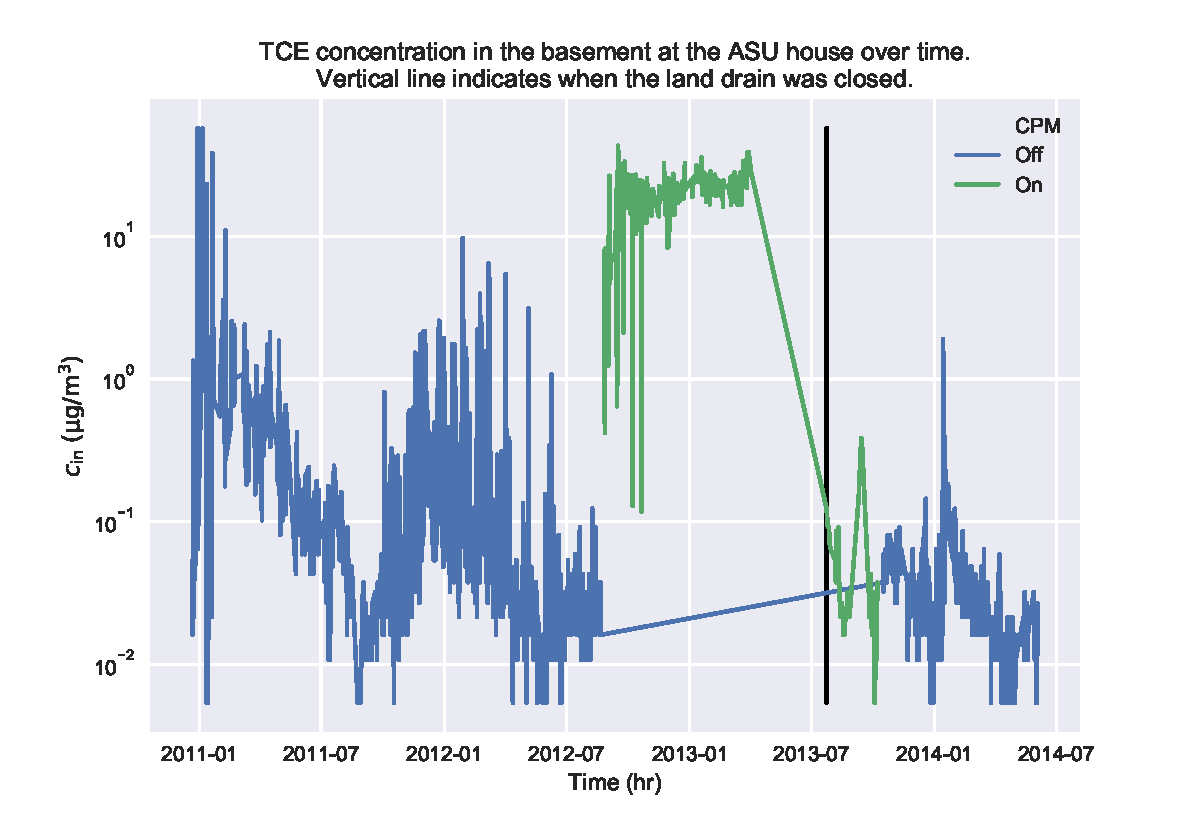
\includegraphics[width=0.75\textwidth]{asu_indoor_concentration.pdf}
    \caption{The temporal variability of indoor air contaminant concentrations recorded at the ASU house. Measurements were taken in the basement. The periods were the CPM system was on and off are marked.}
    \label{fig:asu_indoor_concentration}
  \end{subfigure}
  \begin{subfigure}[t]{\textwidth}
    \centering1
    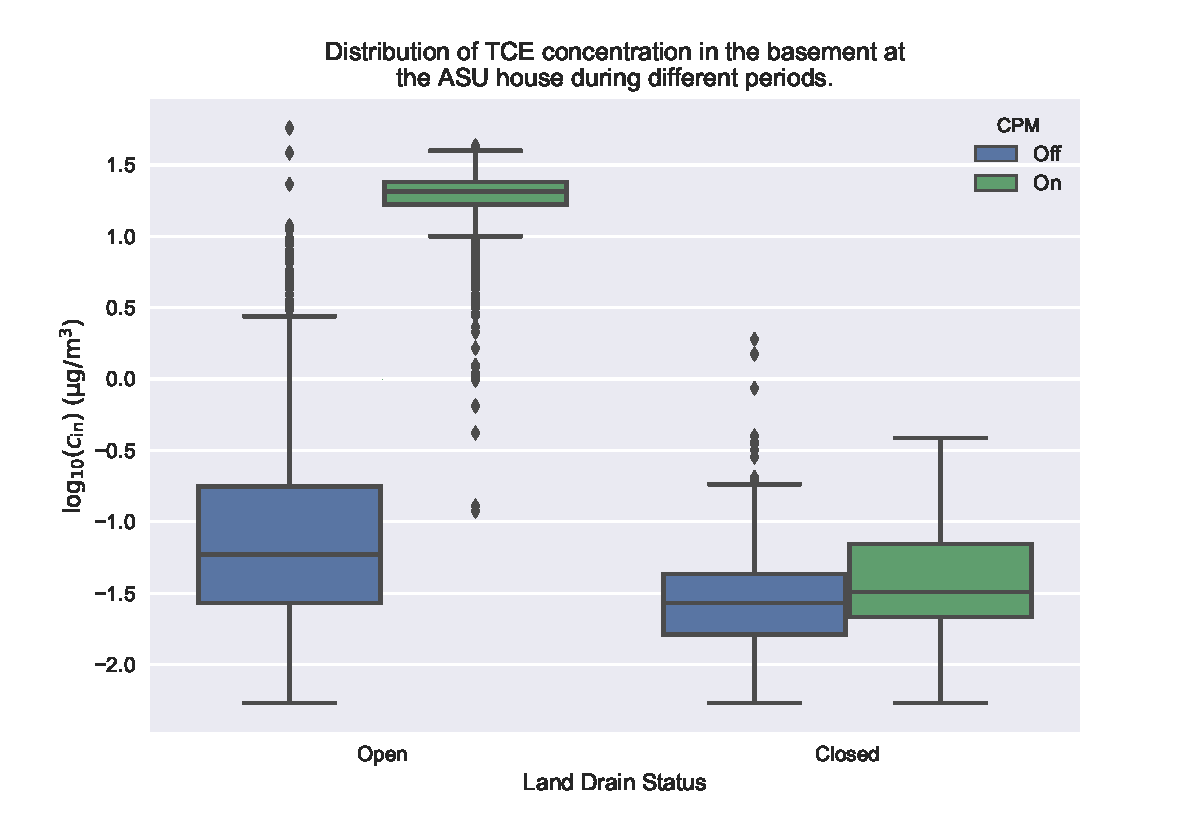
\includegraphics[width=0.75\textwidth]{asu_boxplot_concentration.pdf}
    \caption{Boxplot showing the log-10 transformed TCE concentrations at the ASU house. The CPM and natural periods, and the period before and after the land drain was closed are considered separately. The box signifies the interquartile range (IQR) of values, with the central line representing the median value, and the top and bottom of the box are the \nth{25} and \nth{75} percentiles. The whiskers extend to 1.5 times the IQR. Markers indicate outlier data points that fall outside the whiskers.}
    \label{fig:asu_concentration_boxplot}
  \end{subfigure}
  \caption{}
\end{figure}

The land drain was closed towards the later part of the CPM study, which lead to a significant decrease in indoor contaminant concentration.
This effect can be seen in Figure \ref{fig:asu_indoor_concentration}, which shows the log-10 transformed indoor contaminant concentration for the entire study duration.
Here the pre- and post-CPM periods are marked by colors, and the closing of the land drain by the black vertical line.
Notice how the temporal variability in indoor contaminant concentration decrease significantly after the closing of the land drain.\par

\begin{figure}[htb!]
  \centering
  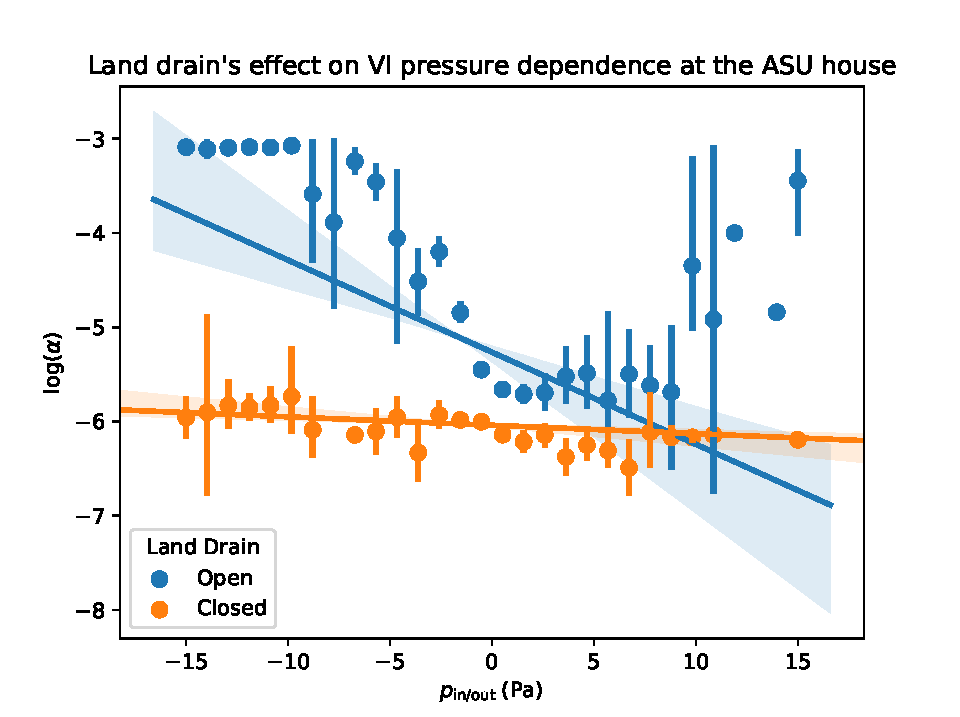
\includegraphics[width=0.75\textwidth]{asu_pressure_dependence.pdf}
  \caption{Regression plot showing the indoor/outdoor pressure difference dependence on indoor air concentration. Here the indoor air concentration is normalized to the groundwater source concentration, i.e. attenuation factor, and log-10 transformed. Data is placed in evenly spaced (but not sized) bins. The bars indicate the 95\% confidence intervals.}
  \label{fig:asu_pressure_dependence}
\end{figure}

Figure \ref{fig:asu_concentration_boxplot} shows the same data, i.e. the log-10 transformed indoor contaminant concentration, but as a boxplot instead of a timeseries plot.
Here the colored box represents the interquartile range (IQR) of the distribution - the middle line is the \nth{50} or median value, while the top and bottom of the represent the \nth{75} and \nth{25} percentile values.
The whiskers are the extent of the dataset, while "outlier" points are given by the dots, here formally defined as data lying 1.5 times outside the IQR; these are "real" data points but simply plotted as outliers not to skew the IQR.
This figure again reinforces the significant effect that the land drain preferential pathway had on the temporal indoor contaminant concentration variability at the ASU house.\par

In the VI field, it is widely held that the building pressurization relative to the ambient outdoor is a key driver of contaminant entry into VI impacted building.
Since building pressurization fluctuations can occurs rapidly, this is a prime factor for investigating the transport dynamics of the preferential pathway.
Figure \ref{fig:asu_pressure_dependence} considers the relationship between the indoor air concentration and building pressurization, specifically indoor/outdoor pressure difference, for the periods when the preferential pathway was open and closed.
This clearly shows the dramatic change in sensitivity of the indoor contaminant concentration to building pressurization after the closing of the preferential pathway, which is not only apparent from visual inspect but from the change in the Pearson's r values for the considered periods.
Pearson's r essentially tells us how linear correlation between two datasets; a value of 1 indicates that there is a perfect positive linear relationship, and -1 a perfectly negative linear relation.
In our context, a negative value indicate that a decrease in building pressurization leads to an increase in indoor contaminant concentration, which makes sense as contaminant entry rates into the house would increase as it is further depressurized.\par

The question then becomes why this fundamental shift in the relationship between building pressurization and indoor contaminant concentration occurred, and how it relates to temporal variability in indoor contaminant concentration.
Answering this is one of the primary objectives of this chapter, which will be done by developing a numerical model of a VI site that is \textit{similar} to the ASU house, and in combination with comparison to the field data, will give insights how a preferential pathway can fundamentally alters contaminant transport at a VI site.
We will also explore how such a preferential pathway can significantly contribute to the spatial variability contaminant concentration, in particular in the near sub-surface region.\par

\subsection{EPA Duplex}

The EPA duplex was, similarly to the ASU house, a highly detailed VI study; Figure \ref{fig:indie_house} shows a photo of the site.
Here the indoor contaminant concentrations of TCE, PCE, chloroform, and radon were measured in different floors of each side of the duplex, as well as in different locations and depths in the subsurface and groundwater - these sampling location ports, as well as a floorplan of the duplex can be seen in Figure \ref{fig:indie_floorplan}.
These sampling ports also allowed pressure differences between different locations to be measured.
Metrological data was collected throughout the study period, which lasted for around 2.5 years, and included indoor and outdoor temperatures, wind speed and direction, precipitation, and recorded snow coverage\cite{u.s._environmental_protection_agency_assessment_2015}.
The data from this site is publicly available online\cite{noauthor_indianapolis_nodate}.\par

\begin{figure}[htb!]
  \centering
  \begin{subfigure}[t]{0.35\textwidth}
    \centering
    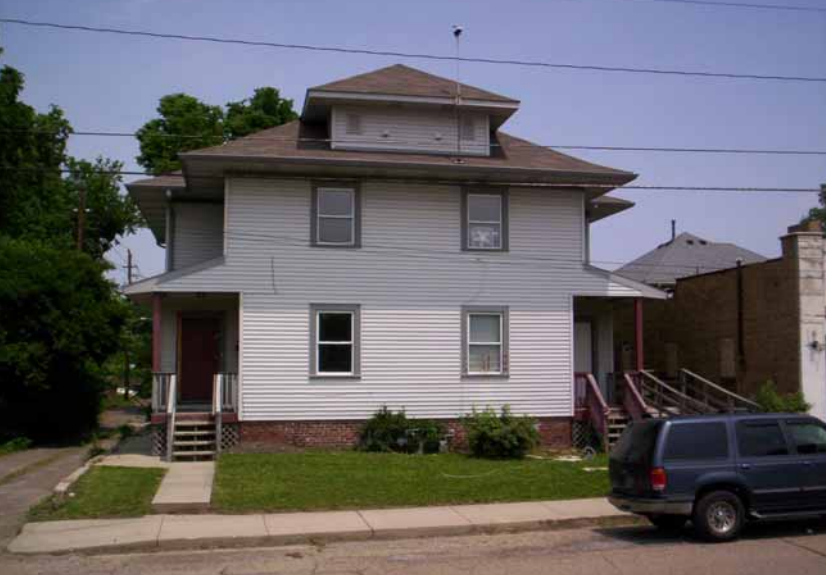
\includegraphics[width=\textwidth]{indianapolis_house.png}
    \caption{Photo of the EPA duplex.}
    \label{fig:indie_house}
  \end{subfigure}
  \begin{subfigure}[t]{0.60\textwidth}
    \centering
    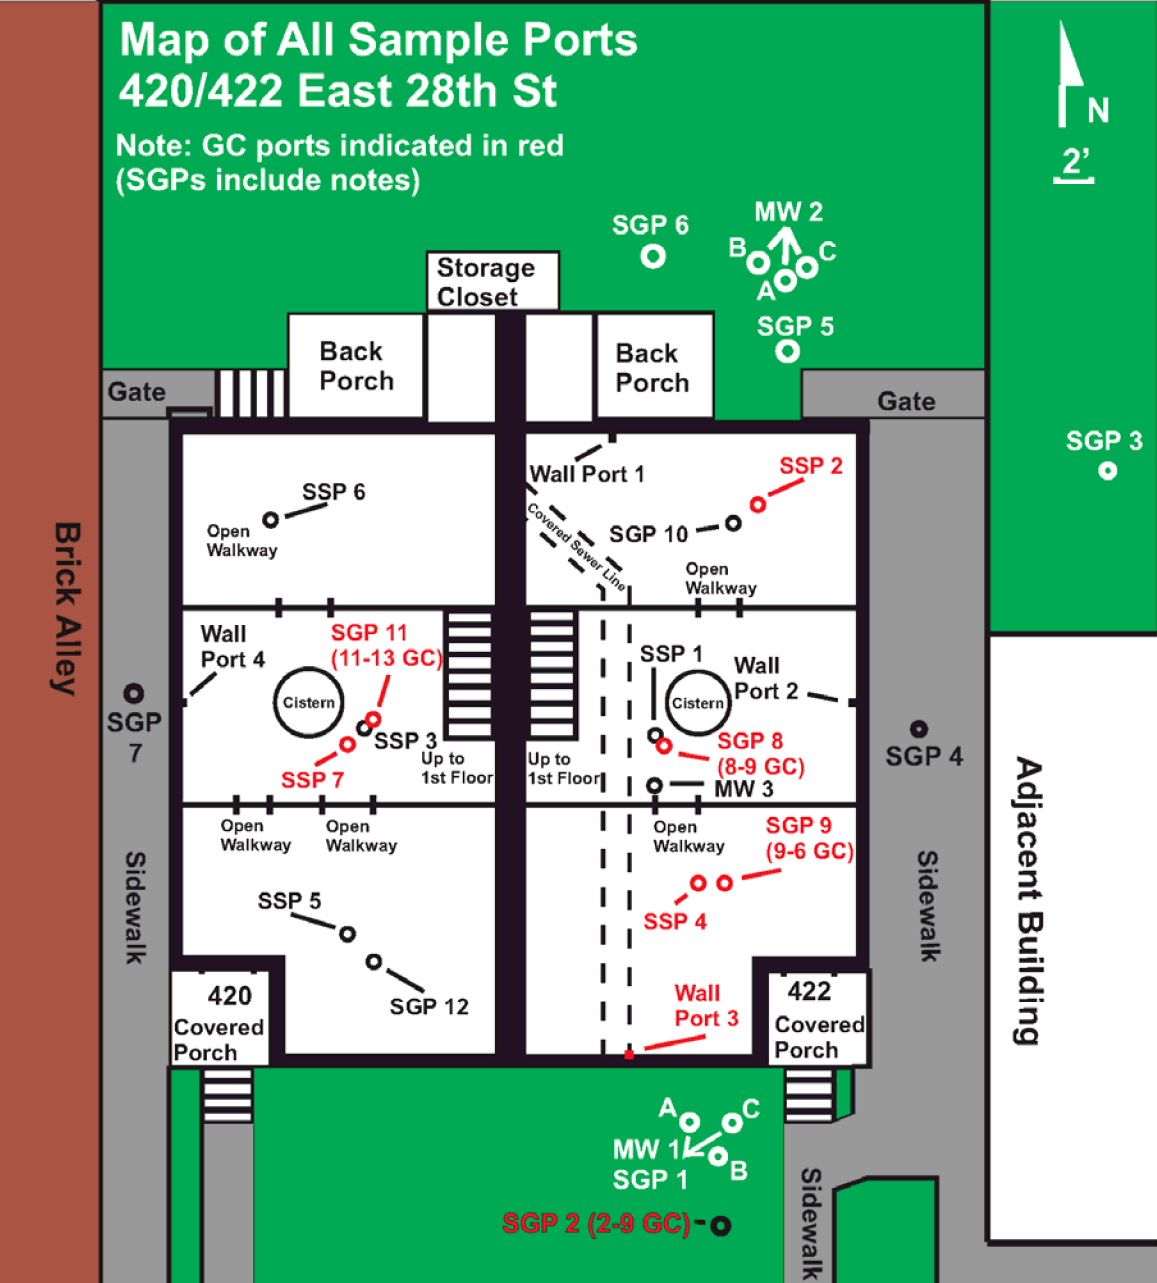
\includegraphics[width=0.45\textwidth]{indianapolis_floorplan.png}
    \caption{Birdseye view of the EPA duplex, listing all the sampling location ports.}
    \label{fig:indie_floorplan}
  \end{subfigure}
  \caption{}
\end{figure}

The was likewise characterized by significant temporal variability in indoor contaminant concentrations, which can be seen in Figure \ref{fig:indie_variability}.
This variability was not as significant as was recorded at the ASU house, but substantial nonetheless.
Understanding the observed variability was a major focus of this study, but additionally the researchers sought to evaluate the efficacy of a subslab depressurization (SSD) system.
A SSD system depressurizes the subslab region, which diverts contaminant vapors from entering the structure into a pipe placed through the foundation slab, which then are expelled into the atmosphere\cite{u.s._environmental_protection_agency_assessment_2015}.
There are many different possible configurations of these pipes, and their design is its own research topic, one which will not be addressed in this work.
However, it is useful to know, and we will only consider data before the implementation of the SSD system.
It should also be noted that only one side of the duplex was heated, and we will only consider data from this side.\par

\begin{figure}[htb!]
  \centering
  \begin{subfigure}[b]{\textwidth}
    \centering
    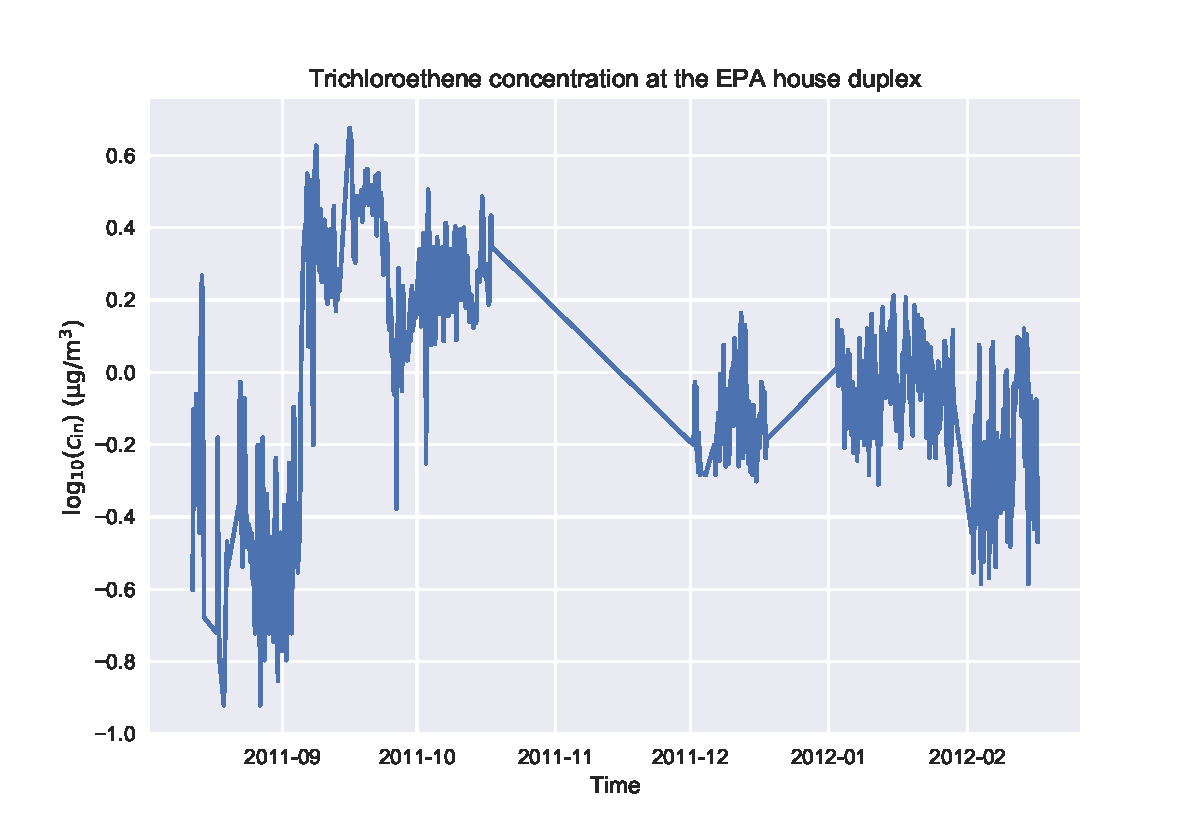
\includegraphics[width=0.75\textwidth]{indie_concentration_time_series.pdf}
    \caption{Time series plot of the indoor TCE concentration in the heated side of the EPA duplex. Only the period before the SSD system was turned on considered.}
    \label{fig:indie_time_series}
  \end{subfigure}
  \begin{subfigure}[b]{\textwidth}
    \centering
    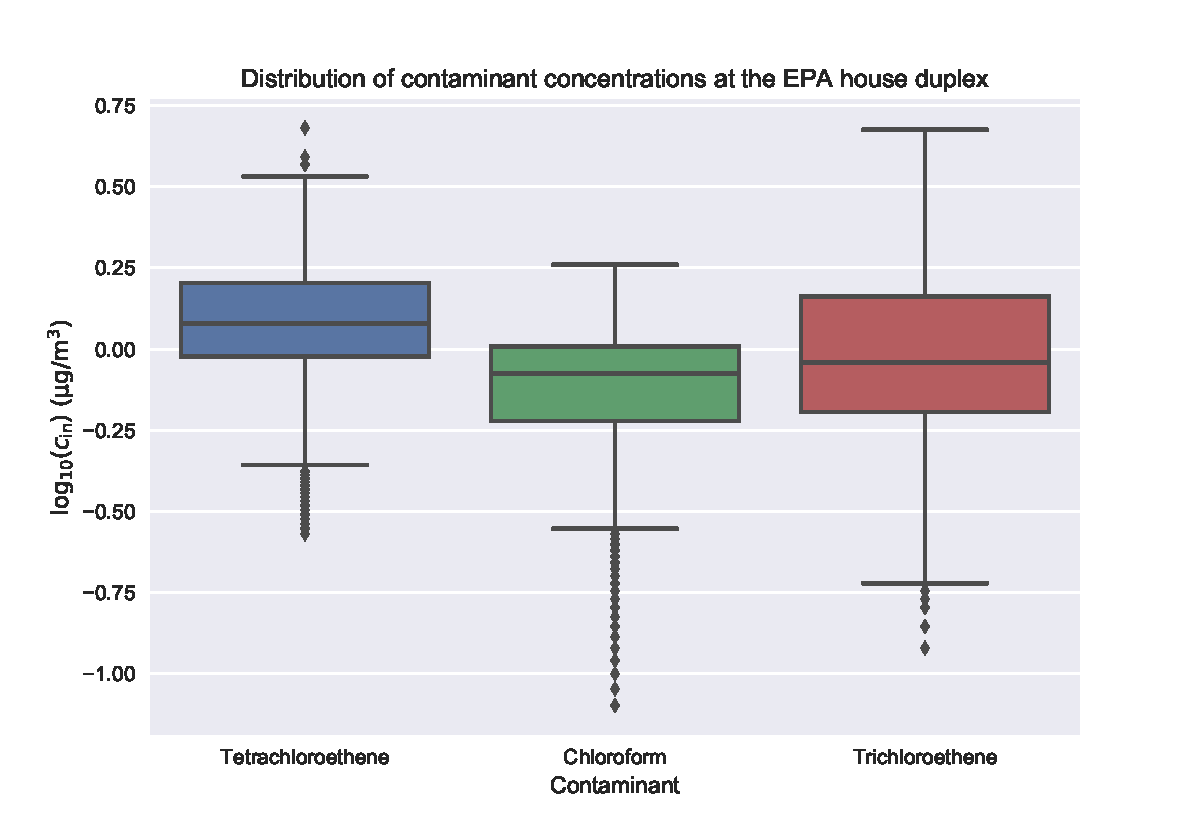
\includegraphics[width=0.75\textwidth]{indie_concentration_boxplot.pdf}
    \caption{Boxplot showing the distribution of log-10 transformed indoor concentration of three different contaminants in the heated side of the EPA duplex. The box is the interquartile range, with the line in the middle representing the median, and the top and bottom of the box representing the \nth{75} and \nth{25} percentiles respectively. The whiskers denote the extent of the data, with the points classified as "outliers", and are defined to be 1.5 times the IQR range.}
    \label{fig:indie_boxplot}
  \end{subfigure}
  \caption{}
  \label{fig:indie_variability}
\end{figure}

Like the ASU house, it was later determined that a sewer preferential pathway existed at the site.
This preferential pathway seemingly played a very different role than the one found at the ASU house, and different in primarily two ways:
\begin{enumerate}
  \item Infiltration of contaminant vapors did not occur near the duplex, but instead occurred a few blocks away - at the site of an old dry cleaner.
  \item Communication between this preferential pathway and the indoor environment does not seem to have been as strong; the researchers believe that this may be due to the poor condition of the sewer pipe, which may have leaked somewhere along its path.
\end{enumerate}
The first of these points was demonstrated by \citeauthor{mchugh_evidence_2017}\cite{mchugh_evidence_2017}, which tracked contaminant vapors along the length of the sewer system.
The second point, or rather the evidence that communication between the indoor environment and the preferential pathway may not have been so strong is indicated by the lower temporal indoor contaminant concentration variability.
It is also indicated by the weaker association between indoor contaminant concentration and the indoor/outdoor pressure difference, which can be seen in Figure \ref{fig:indie_pressure_dependence}; this weaker association is indicated by the smaller Pearson's r values compared to the ones at the ASU house before he closing of that preferential pathway.\par

\begin{figure}[htb!]
  \centering
  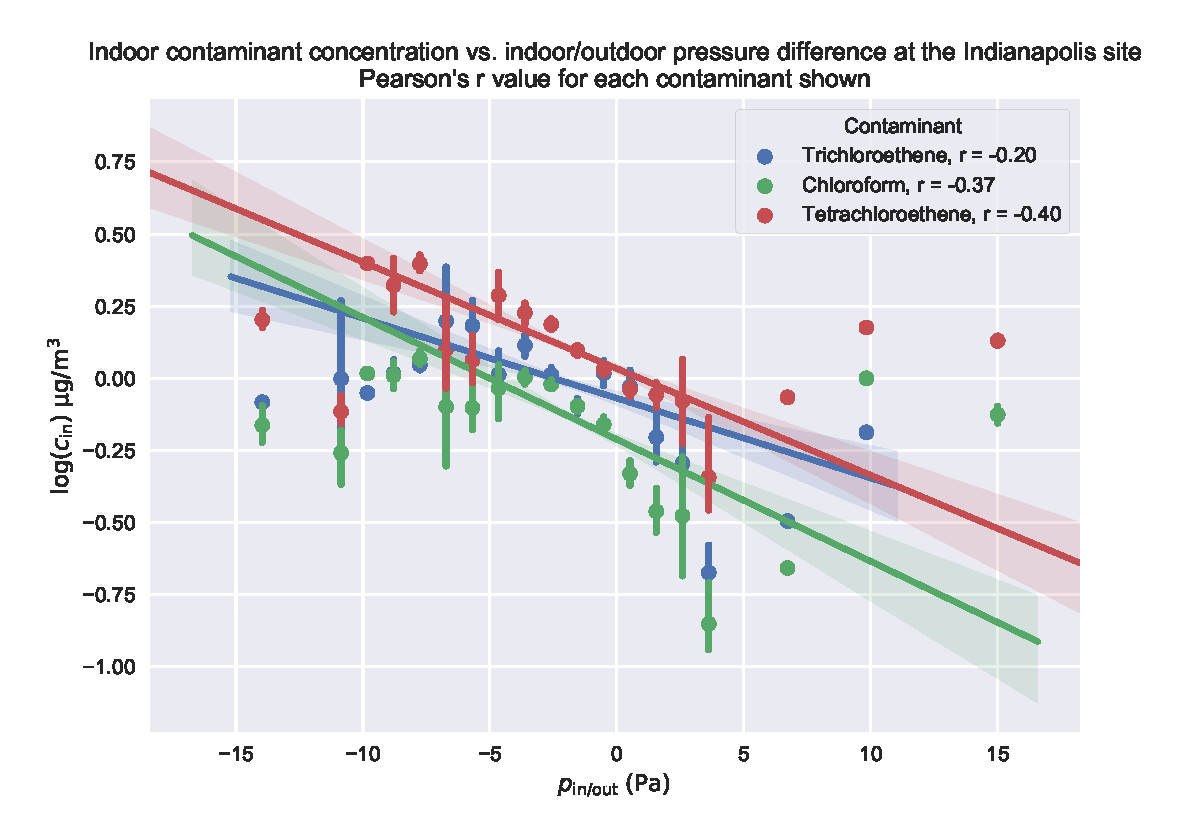
\includegraphics[width=0.75\textwidth]{indie_pressure_dependence.pdf}
  \caption{Relationship between indoor/outdoor pressure difference and indoor contaminant concentration of three contaminants - TCE, PCE, and chloroform at the EPA duplex.}
  \label{fig:indie_pressure_dependence}
\end{figure}

Unfortunately, the EPA duplex preferential pathway is less well characterized, and its influence was never removed.
This makes it difficult to assess how it contributed to overall VI at the site, or the observed temporal variability in indoor contaminant concentrations.
However, it is possible to explore if the preferential pathway leaked somewhere near the site - which likewise will be a focus in this chapter.\par

Determining leakiness of the preferential pathway will be done by performing a kriging analysis of the measured soil-gas contaminant concentrations.
Kriging is a type of interpolation technique which allows sparse data to be interpolated in multiple dimensions; ideal for interpolating soil-gas contaminant concentration in the soil surrounding the duplex.
This way we can visually inspect the interpolated soil-gas contaminant concentration for "hot spots", which could indicate where such a leak might be.\par
